\documentclass[__main__.tex]{subfiles}

\begin{document}

\qtitle{Э}{11}
Найдите магнитное поле постоянного кругового (радиус $a$) тока $I$ на его оси. Чему равен магнитный момент этого витка с током?\\ 

$$
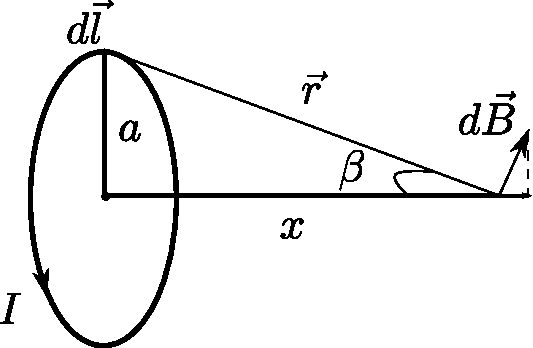
\includegraphics[scale=0.8]{img/e11.pdf}
$$

Найдем $\vec{B}$ на оси кругового тока, на расстоянии $x$ от плоскости, в которой лежит контур. Векторы $d\vec{B}$ перпендикулярны к плоскостям, проходящим чрез соответствующие $d\vec{l}$ и $\vec{r}$. Следовательно, они образуют симметричный конический веер. Из соображений симметрии можно заключить, что результирующий вектор $\vec{B}$ направлен вдоль оси тока. Каждый из составляющих векторов $d\vec{B}$ вносит в результирующий вектор вклад $d\vec{B}_{||}$, равный по модулю $dB\sin\beta=dB\dfrac{a}{r}$. Угол между $d\vec{l}$ и $\vec{r}$ прямой, поэтому 
\begin{gather*}
dB_{||}=dB\frac{a}{r}=\frac{\mu_0}{4\pi}\frac{Idl}{r^2}\frac{a}{r}=\frac{\mu_0}{4\pi}\frac{Iadl}{r^3}
\end{gather*}
Проинтегрировав по всему контуру и заменив $r$ на $\sqrt{a^2+x^2}$, получим:
\begin{gather*}
B=\int dB_{||} = \frac{\mu_0}{4\pi}\frac{Ia}{r^3}\int dl = \frac{\mu_0}{4\pi}\frac{Ia}{r^3} 2\pi a=\frac{\mu_0}{4\pi}\frac{2\pi a^2I}{(a^2+x^2)^{3/2}}
\end{gather*}
Магнитный момент этого контура:
\begin{gather*}
p_m=\pi a^2I
\end{gather*}

\end{document}